\chapter{\IfLanguageName{dutch}{Stand van zaken}{State of the art}}%
\label{ch:stand-van-zaken}

% Tip: Begin elk hoofdstuk met een paragraaf inleiding die beschrijft hoe
% dit hoofdstuk past binnen het geheel van de bachelorproef. Geef in het
% bijzonder aan wat de link is met het vorige en volgende hoofdstuk.

% Pas na deze inleidende paragraaf komt de eerste sectiehoofding.

%Dit hoofdstuk bevat je literatuurstudie. De inhoud gaat verder op de inleiding, maar zal het onderwerp van de bachelorproef *diepgaand* uitspitten. De bedoeling is dat de lezer na lezing van dit hoofdstuk helemaal op de hoogte is van de huidige stand van zaken (state-of-the-art) in het onderzoeksdomein. Iemand die niet vertrouwd is met het onderwerp, weet nu voldoende om de rest van het verhaal te kunnen volgen, zonder dat die er nog andere informatie moet over opzoeken \autocite{Pollefliet2011}.
%
%Je verwijst bij elke bewering die je doet, vakterm die je introduceert, enz.\ naar je bronnen. In \LaTeX{} kan dat met het commando \texttt{$\backslash${textcite\{\}}} of \texttt{$\backslash${autocite\{\}}}. Als argument van het commando geef je de ``sleutel'' van een ``record'' in een bibliografische databank in het Bib\LaTeX{}-formaat (een tekstbestand). Als je expliciet naar de auteur verwijst in de zin, gebruik je \texttt{$\backslash${}textcite\{\}}.
%Soms wil je de auteur niet expliciet vernoemen, dan gebruik je \texttt{$\backslash${}autocite\{\}}. In de volgende paragraaf een voorbeeld van elk.
%
%\textcite{Knuth1998} schreef een van de standaardwerken over sorteer- en zoekalgoritmen. Experten zijn het erover eens dat cloud computing een interessante opportuniteit vormen, zowel voor gebruikers als voor dienstverleners op vlak van informatietechnologie~\autocite{Creeger2009}.

In dit hoofdstuk wordt eerst bekeken wat een API juist is. De precieze werking van REST alsook van gRPC worden daarna grondig onderzocht met extra aandacht voor
eventuele aspecten die de performantie kunnen beïnvloeden. Tot slot worden beide technologieën ook met elkaar vergeleken.

\section{API}

Een application programming interface, vaker API genoemd, is een connectie tussen computers of applicaties.
Een API-specificatie verwijst dan weer naar een standaard die beschrijft hoe een dergelijke interface of connectie moet werken.
Van een applicatie die deze standaard volgt, wordt gezegd dat ze een API blootstelt. API kan verwijzen naar de standaard zelf of naar de applicatie die deze implementeert.
Zeer vaak wordt, wanneer naar een API wordt verwezen, een web API bedoeld. Een web API bewerkstelligt de communicatie, die via het internet verloopt, tussen applicaties.\\

REST en RPC zijn beiden API's en meer specifiek web API's in die zin dat ze specificaties zijn die aangeven hoe een connectie tussen twee systemen kan geïmplementeerd worden.
gRPC daarentegen is een implementatie van Google van de RPC specificatie.\\

API's worden ontzettend veel gebruikt waardoor ze ook zeer belangrijk zijn. Elke website, elke browser, maar ook nagenoeg elk apparaat dat met internet verbonden is,
de zogenaamde smart devices, maakt er gebruik van. De evolutie in de technologische ontwikkeling is van die aard dat er steeds meer apparaten verbonden zijn met elkaar
en dat deze apparaten ook steeds vaker, en tevens grotere, datasets versturen. Aan de hand van de API's zijn consumenten in staat deze apparaten aan te sturen en te monitoren
en daarnaast zorgen ze voor een massa aan data die direct bruikbaar is of het potentieel heeft om bruikbaar te worden. Data die, vanuit het standpunt van de producenten, niet mag verloren gaan.\\

Het wijdverspreide gebruik van API's, de constante toename van dat gebruik, en zeker ook de toename van de grootte van de data die wordt verzonden, toont
direct aan dat performantie een zeer belangrijk punt is. Elke software-ontwikkelaar of -architect dient hier rekening mee te houden, en moet het ontwerp van de
applicatie alsook de keuze voor bepaalde technologieën afstemmen op de noden van de applicatie en haar gebruikers.
~\autocite{cleo}

\section{REST}

Representational State Transfer, vaker benoemd door middel van het acronym REST, is een type van web API. Deze technologie wordt zeer vaak gebruikt om webservices te bouwen.
Dit zijn applicaties die diensten of data als web resources aanbieden. Door middel van een REST API kan de client om deze resources vragen zonder verder
begrip van de interne werking van de provider. De server reageert dan door een response te versturen met een status code en met de resource in JavaScript object Notation (JSON),
Extensible Markup Language (XML) of andere tekstindelingen. Een web resource is eigenlijk alles waarmee een client op het web kan communiceren.
Het kan betrekking hebben op een bestand, afbeelding, HTML of video. Een resource kan ook een service zijn zoals Google Maps of een financiële dienst.
De API-ontwikkelaars moeten de beslissing maken welke resources ze ondersteunen voor de response.
De API moet de mogelijkheid hebben om de response op te maken op basis van de behoefte van de client.
~\autocite{uptrends}
~\autocite{guru99-webservices}\\

Opdat een API als RESTfull kan worden beschouwd moet het aan enkele kenmerken voldoen.\\
Ten eerste dient het, voor de communicatie, gebruik te maken van het HTTP 1.1 protocol. Het protocol, dat zich in de applicatie laag situeert,
bepaalt dat de client een request, met tekst als vorm, verstuurt naar de server waarop die de gevraagde gegevens terugzendt.
HTTP specificeert verschillende soorten requests methods waaronder GET, POST, PUT en DELETE. Een REST API kan van al deze methods gebruik maken en zal dat
hoogstwaarschijnlijk ook doen. HTTP 1.1 houdt een TCP-connectie open tot er uitdrukkelijk opdracht gegeven wordt om deze te sluiten.
Dit geeft een enorme performantie winst t.o.v. HTTP 1.0. Het nadeel van deze uitdrukkelijke opdracht is dat een wachtende request alle achterliggende requests kan blokkeren.
Extra TCP-connecties kunnen hier een oplossing bieden, deze zijn echter ook gelimiteerd.
~\autocite{w3Protocol}\\
Als tweede kenmerk moet een REST API stateless zijn. Dit houdt in dat er geen informatie zal worden opgeslagen tussen requests door.
De API zal de verbinding tussen server en client verbreken nadat de server een resource in de vorm van een response heeft doorgezonden aan de client.
De API behandelt zo elke request los van een eventuele vorige request. Dit vermindert de hoeveelheid geheugen die een server nodig heeft en verhoogt de
kans op een succesvoller antwoord omdat de server geen extra stappen moet nemen om oude data op te zoeken.\\
Het derde kenmerk voorziet erin dat de verstuurde data cacheable moet zijn. De client weet namelijk a.d.h.v het type van REST request,
meer specifiek de request method, dat hij verzonden heeft wat voor antwoord hij kan verwachten.\\
De vierde eigenschap bestaat uit de verplichting een uniforme interface tussen componenten te voorzien zodat data kan verzonden worden in een standaard vorm.\\
Het vijfde kenmerk specificeert dat het niet noodzakelijk mag zijn dat de client kennis heeft van de verdere werking van de server(s) buiten de vorm van de communicatie zelf.\\
Tot slot laat het zesde, en enige optionele, kenmerk toe om executeerbare code te verzenden indien zo verzocht wordt door de client.
~\autocite{redhat}\\

REST API's zijn flexibel. Ze kunnen requests van verschillende types aan alsook kunnen ze data versturen in verschillende formaten.
Webapplicaties groeien aangezien er telkens meer resources worden toegevoegd. Een REST API zal deze toenemende hoeveelheid van variërende requests snel kunnen behandelen.\\

Een REST API spitst zich steeds toe op het domein dat het als resource zal aanbieden.
Dankzij deze focus alsook de uniforme manier van werken is het voor de client duidelijk welke functionaliteiten hij kan aanroepen en hoe dat te doen.
~\autocite{jscrambler}
~\autocite{hubspot}
~\autocite{HTTP1.1vsHTTP2}\\

Afhankelijk van de taal waarin, de tussen server en client, verstuurde data zich bevindt, alsook de programmeertaal van beide applicaties,
zal er bij zowel de client als de server een serialisatieproces moeten plaatsvinden. Er zijn verschillende libraries die de serialisatie kunnnen verzorgen,
zo kan er bij Java gebruik gemaakt worden van b.v. Jackson~\parencite{jackson} \newline
Bij de client zal gebruik moeten gemaakt van documentatie van de serverapplicatie of door de endpoints manueel aan te roepen
en zo op basis van de response de mapping voor het serialisatieproces op te maken. Het schrijven van de documentatie,
het creëren van de code in de client om het REST API van de server aan te roepen en zelfs de code in de server kan automatisch gegenereert worden dankzij
handige hulpmiddelen zoals b.v. Swagger~\parencite{swagger}.\\

Tijdens de levensduur van een API is het bijna onvermijdelijk dat er aanpassingen gebeuren. Sommige van deze aanpassingen, zoals het toevoegen van een extra veld aan een object,
hebben geen invloed op eventuele clients en worden daarmee non-breaking changes genoemd. Andere aanpassingen, de zogenaamde breaking changes, hebben als gevolg dat er
fouten kunnen optreeden bij clients. Zo kan het verwijderen van een veld uit een object plots een error veroorzaken bij
een client die het API aanroept en verwacht dat dit veld aanwezig is. In REST API's wordt, wanneer een breaking change geimplementeerd wordt,
meestal gewerkt met een versie verhogen, ook version bump genoemd. De client moet dan bij elke request aangeven welke versie er wordt aangeroepen.
Dit kan door een aparte url per versie, door het versienummer mee te geven in een specifieke request header of door de versie aan de Accept header toe te voegen.
Deze verschillende versies kunnen in dezelfde applicatie gesupporteerd worden of er worden verschillende versies van de applicatie gedeployed.
~\autocite{restversion}\\

\section{gRPC}

Een RPC API stelt een client in staat om op afstand een serverfunctie aan te roepen, zonder dat de client zich verder bewust hoeft te zijn van de interne werking
van de server of de implementatie van de functie.
RPC maakte in het verleden, net zoals REST, gebruik van het HTTP-protocol. De XML-RPC alsook de JSON-RPC implementaties zijn hier voorbeelden van.
Zij maken gebruik van de HTTP request methods GET en POST. De eerste voor het ophalen van data en de tweede voor alle andere functies.\\

De functies van een RPC API kunnen specifiek gericht zijn op de functionaliteit die ze implementeren en daarmee potentieel ook lichtgewicht zijn.
De client moet enkel de naam van de functie specificiëren en de vereiste data meegegeven. De response zal ook enkel de data bevatten die door de server nodig wordt geacht.
Wanneer de functies zodanig toegespitst zijn op een functionaliteit wordt er aan de consumer inzicht gegeven over de interne werking van de server,
alsook dient de client vaak kennis te hebben over die interne werking om de functies te kunnen gebruiken.
~\autocite{altexsoft}\\

Google Remote Procedure Calls (gRPC) is de implementatie van Google van het RPC API.\\
Een eerste groot verschil tussen RPC en de implementatie van Google is dat gRPC gebruik maakt van het HTTP2-transportprotocol.
HTTP2 werd in 2015 uitgebracht. De doelstellingen bij het ontwikkelen van deze nieuwe versie van het protocol waren vooral toegespitst op performantie.
Hiebij werden enkele nieuwe functies en kenmerken ontwikkeld. Request multiplexing laat toe om requests simultaan te laten gebeuren.
Dankzij Request prioritization kan een prioriteit gegeven worden aan requests. Requests en responses worden nu automatisch gecomprimeerd i.t.t. op
uitdrukkelijk verzoek. De mogelijkheid om de verbinding te resetten werd toegevoegd. Daarenboven kan de server ook proactief resources verzenden naar de
cache van clients via de zgn. server push functie. En tot slot is HTTP 2 een binair protocol t.o.v. het op gewone tekst gebaseerde HTTP 1.1 protocol.
~\autocite{baeldung}\\

Het verplicht gebruik van HTTP2 komt echter ook met het nadeel dat gRPC hierdoor niet ondersteund wordt door de hedendaagse browsers.
Voor gRPC moeten er b.v. trailing headers blootgesteld worden welke door browser steeds verborgen worden. Een oplossing hiervoor is het gebruik van een proxy welke
door middel van een normale HTTP request communiceert met de browser en dan de request via gRPC naar de server doorgeeft.
~\autocite{altexsoftgrpc}\\
~\autocite{yukutakahashi}\\

gRPC gebruikt geen JSON, XML, of zelfs enig ander teksformaat, maar protocol buffers, ook protobuf genoemd. Protobuf is zodanig geformatteerd dat het niet leesbaar is
voor het menselijk oog. Berichten worden verkleint tot een binair formaat waardoor de snelheid van data transacties hoger zou liggen. gRPC heeft een ingebouwde
protoc-compiler voor het genereren van API-aanroepen en kan zo makkelijk inspelen op vele programmeertalen.
Ondanks deze compiler is een implementatie vaak nog tijdrovender dan alternatieve API's.
~\autocite{googleprotobufguide}\\
~\autocite{dreamfactory}\\

gRPC wordt steeds populairder dankzij de opkomst van microservices. Dit zijn services die onafhankelijk van elkaar worden gebouwd en geïmplementeerd om
zo tot een gehele toepassing te komen. Bij een fout in één van de services zal dit niet de hele app gaan verstoren.
Om goed met elkaar te kunnen communiceren zijn er dus goed gedefineerde API-contracten nodig.
~\autocite{microsoft}\\

Dankzij de eerder vermelde multiplexing kunnen meerdere dingen tegelijk gebeuren, meerdere requests tegelijk worden verzonden, bij één enkele connectie.
Wat hier zeker naar voor treedt is het bidirectioneel streamen. Zowel de client als de server sturen berichten naar elkaar op hetzelfde moment zonder te moeten wachten
op een antwoord. Een client kan zelfs een request annuleren als er geen response meer nodig is van de server.
~\autocite{freecodecamp}\\

Bij gRPC moet er ook rekening gehouden worden met versionering, breaking changes kunnen tot fouten bij clients kunnen leiden.
Bij protobuf zijn er binaire breaking changes die het protoc niet breken maar waarbij de clients wel moeten aangepast worden en protocol breaking changes
die ook effectief het protocol breken en tot gevolg geven dat de clients de status ``UNIMPLEMENTED`` verkrijgt. De versienummer wordt toegevoegd aan
het .proto bestand. Meerdere versies supporteren houdt in dat de applicatie zal moeten gedupliceerd worden.

~\autocite{grpcversion}\\

\section{REST vs gRPC}

Bij het overlopen van de kenmerken van REST en gRPC komen direct enkele belangrijke verschillen naar boven.
Het feit dat REST werkt met het HTTP 1.1 en gRPC met het HTTP 2 protocol heeft ingrijpende gevolgen. HTTP 2 heeft alle mogelijkheden van het 1.1 protocol,
maar voegt daar de hierboven opgesomde functionaliteiten aan toe (Request multiplexing, Request prioritization, Automatic compressing,
Server push en haar binaire vorm). Deze bijkomende functionaliteiten zijn voornamelijk toegespitst op een verbetering van de performantie en efficiëntie van dataoverdracht.
Daarentegen zorgt het gebruik van HTTP2 door gRPC wel voor het nadeel dat er geen rechtstreekse communicatie met browsers mogelijk is.
~\autocite{cloudflare}
~\autocite{tutsplus}\\

Een tweede belangrijk verschil is zichtbaar bij de protocol buffers van gRPC versus het gewone tekst formaat dat gebruikt wordt bij REST-API's.
Dit verschil bouwt duidelijk ook verder op het voorgaande punt m.b.t. het HTTP 1.1 en HTTP 2 protocol.
Protobuf is gelijkaardig aan JSON in die zin dat het beiden programmeer-taal onafhankelijke data uitwisselings formaten zijn.
Protobug gaat verder dan JSON en is eerder een mechanisme voor het serialiseren en de-serialiseren van data.
JSON is leesbaar voor mensen terwijl het binaire formaat bij Protobuf dat niet is~\parencite{json}
Bij deze protocol buffers wordt de datastructuur éénmaal vastgelegd en gaat de gegenereerde code van gRPC de serialisatie en deserialisatie van de data verzorgen.
Dit serialisatieproces zorgt dat data compact gemaakt wordt voordat ze wordt verzonden wat een performantiewinst zou betekenen. ~\autocite{googleprotobufguide}\\

Daar staat wel tegenover dat de data, zoals vermeld, steeds vooraf gedefinieerd dient te worden.
Het verzenden van dynamische data maakt het voordeel dat bereikt wordt tijdens de serialisatie namelijk ongedaan.\\

REST heeft een grotere simpliciteit dan gRPC. Er is bij REST enkel een http-compatible client nodig om een applicatie te ontwikkelen terwijl
er bij gRPC steeds protobuf nodig is voor het deserialisatieproces. Toch moet er ook rekening gehouden worden met het feit dat bij REST,
afhankelijk van de programmeertaal waarme gewerkt wordt, ook een serialisatieproces nodig is. Zo words bij Java ondermeer gebruik gemaakt van Jackson.\\
~\autocite{jackson}

Beide technologiën laten toe de server en client volledig van elkaar te scheiden waardoor ze goed schaalbaar zijn.

Breaking changes zijn zowel voor gRPC als REST een mogelijks probleem voor de clients waardoor er met versionering moet gewerkt worden.
REST laat toe verschillende versies te supporteren met één applicatie die bepaalde logica herbruikt. Bij gRPC daarentegen wordt code gegenereerd op basis van
het schema waardoor er duplicatie zal zijn bij verschillende versies.
~\autocite{grpcversion}

gRPC is minder wijdverspreid dan REST. Dit geeft voordelen voor REST, gaande van gekende best practices, oplossingen voor allerhande problemen
tot simpelweg ontwikkelaars met ervaring vinden. Kijk maar naar het aantal vragen op stackoverflow voor REST, op vandaag 93164 ~\parencite{stackrest},
versus die voor gRPC, op heden 6025 ~\parencite{stackgrpc}. De grafiek in figuur 2.1 toont wel aan dat het aantal vragen over gRPC in stijgende lijn gaat terwijl
dit voor REST licht dalend is.
\begin{figure}[ht]
    \centering
    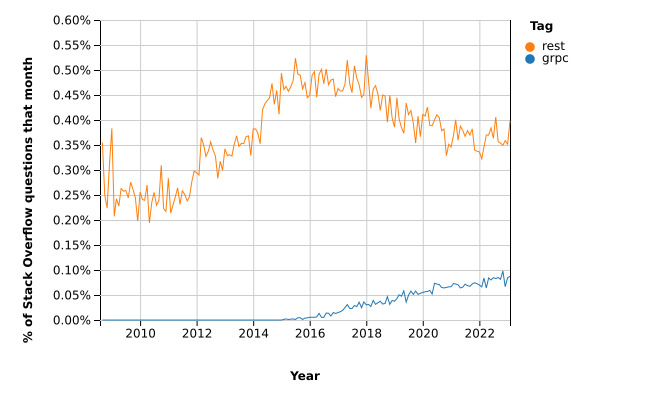
\includegraphics[width=1.0\linewidth]{stackoverflowgrpcrest}
    \caption{Percentage Stack Overflow vragen per maand voor gRPV en REST,\newline
        https://insights.stackoverflow.com/trends?tags=grpc\%2Crest}
\end{figure}\\